% LaTeX file for resume 
% This file uses the resume document class (res.cls)
\documentclass[margin,line]{res} 
\usepackage{hyperref}
\usepackage[export]{adjustbox}
\usepackage{wrapfig}
\usepackage{lipsum}



\setlength{\topskip}{0mm}
\setlength{\parindent}{1mm}
\oddsidemargin -.5in
\evensidemargin -.5in
\textwidth=6.0in
\itemsep=0in
\parsep=0in
\topmargin=-0.5in
\topskip=-0.5in
\textheight 9.5in

\newcommand{\MySlogan}[1]{ % Slogan}{optional)
		\large \usefont{OT1}{phv}{m}{n}\hfill \textit{#1}
		\par \normalsize \normalfont}

\newcommand{\MyName}[1]{ % Name
		\Huge \usefont{OT1}{phv}{b}{n} \hfill #1
		\par \normalsize \normalfont}
% the margin option causes section titles to appear to the left of body text 
%\textwidth=5.2in % increase textwidth to get smaller right margin
%\usepackage{helvetica} % uses helvetica postscript font (download helvetica.sty)
%\usepackage{newcent}   % uses new century schoolbook postscript font 

\begin{document} 


% \thispagestyle{empty} % this page has no header  
% \begin{tabular}{@{}p{3.5in}p{3in}}
% {\bf Contact Information:}
% \\39 West Lexington Street, \\803             
% Baltimore, MD, 21201
%  \\{Phone:}  (443) 653-7320 \\
%  {E-mail:}  zahranoorcs1514@gmail.com\\

% \end{tabular}
% \hfill
% 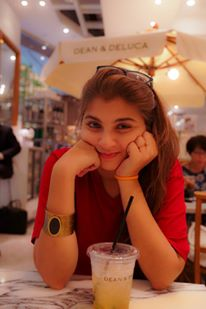
\includegraphics[width=3cm,valign=t]{mypic.jpg}%
% %\name{Zahra Noor\\[12pt]} % the \\[12pt] adds a blank line after name
% \name{\LARGE Zahra Noor}


\begin{wrapfigure}{l}{0.5\textwidth}
	\vspace*{-2em}
	\hspace*{-10em}
		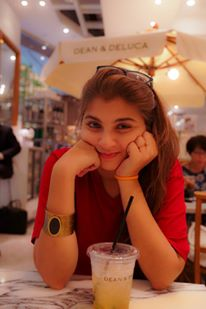
\includegraphics[width=0.15\textwidth]{mypic.jpg}
\end{wrapfigure}

\MyName{Zahra Noor}
% \MySlogan{Curriculum Vit\ae\ (\today)}
\MySlogan{Web Developer}
\MySlogan{\vspace{-0.6in}\begin{flushright}{}{39 West Lexington Street}\\803, Baltimore, MD, 21201 \\
(443) 653-7320\\
E-mail: \href{mailto:zahranoorwd@gmail.com}{zahranoorwd@gmail.com}\\
\MySlogan{Portfolio: \href{https://zahranoorcs.github.io/ZahraPortfolio/}{\bf Click Here}}
\end{flushright}}


\begin{resume} 
 
% \section{\bf Contact Information}
% \vspace{.05in}
% \begin{tabular}{@{}p{3.5in}p{3in}}
% 39 West Lexington Street, \\803             
% Baltimore, MD, 21201
%  \\{Phone:}  (443) 653-7320 \\
%  {E-mail:}  zahranoorcs1514@gmail.com\\

% \end{tabular}

\section{Career Summary}

Front End Web Developer with first hand experience of multi-platform responsive, accessible, usable and adaptive web-design. Experience with Front End (HTML, CSS, JavaScript, Bootstrap, jQuery, AJAX); Back End (SQL, PHP, AngularJS); Content Management Systems (Wordpress, Drupal, Placester, Squarespace) and Design Softwares (Adobe CC). Open to full-time challenging roles, that will allow me to showcase my abilities while also enhancing or building great websites.

\section{Professional \\Experience}

\href{https://www.air.org/}{\noindent\bf American Institutes For Research (AIR)}, Washington, D.C. \hfill{December 2017 -- Present}\\
Web Designer I
\begin{itemize} \itemsep -2pt  % reduce space between items
 \item Responsible for ensuring compliance with WCAG 2.1, WAI-ARIA, HTML5 and web standards to make sure that all the components are accessible by making them perceivable, operable, understandable and robust.
 
 \item Developed a style guide toolkit using fabricator for accessibility developers to reduce overhead due to repetition and complexity. 
 \item Increasing accessibility in AIR assessment and testing products to ensure a user-friendly experience for people with disabilities. 

 \item Collaborating with teams in order to conduct function-based brainstorming for chalking out innovative ways to resolve accessibility bugs.
 \item Active reviewing of websites created by other colleagues and giving feedback for accessibility compliance, usability, design and functionality. 
 \item  Developing demonstrative website mockups using Photoshop.

 %\item Some experience in creating mock-ups and presentations.
 %\item Collaborating with teams in order to conduct function-based brainstorming. 

 \end{itemize}

\href{http://www.rlathome.com/}{\noindent\bf Real Living At Home (RLAH)}, Washington, D.C. \hfill{August 2017 -- November 2017}\\
Web Developer
\begin{itemize} \itemsep -2pt  % reduce space between items
 \item Developing real estate websites to provide agents a platform for displaying their home listings, branding themselves as realtors and providing different home search criteria depending on min and max prices, number of beds and baths, acres and a couple of more factors in websites which make house hunting easy for their customers. 
 \item Utilized HTML, CSS, JavaScript, PHP, Wordpress, Bootstrap, IDX Broker and Placester.
 \item Converting wireframes into Web Pages.
 \item Increasing responsiveness of webpages using Bootstrap.
 \item Testing site functionality and resolving bugs.
 \item Integrating IDX Broker in real estate websites.
 \item Customizing websites according to agents needs.
 \item Capitol Luxury Homes (Wordpress, IDX Broker) \href{http://dev.capitolluxuryhomes.com/}{\bf Website 1}
 \item Capitol Luxury Homes (Placester, IDX) \href{http://bit.ly/2gMSN8T}{\bf Website 2}
 \item THINKTANCK (Placester, IDX Broker) \href{http://justinlevitch2.myrealestateplatform.com}{\bf Website 3}

 %\item Some experience in creating mock-ups and presentations.
 %\item Collaborating with teams in order to conduct function-based brainstorming. 

 \end{itemize}

\href{http://www.datanext.co.jp/en/}{\noindent\bf DataNext Corporation Ltd}, Naha, Okinawa. Japan \hfill{June 2016 -- March 2017}\\
Junior Web Developer
\begin{itemize} \itemsep -2pt  % reduce space between items
 \item Developing a web-based application as a real-time aid for product delivery staff to generate reports and for managers to monitor delivery schedule, delivery location, work efficiency etc. using Laravel MVC as the framework.
 The application included additional features for delivery staff to make their delivery schedule, routing and sorting more easy.
 \item Used geolocation API for user localization.
 \item Utilized HTML, CSS, JavaScript, PHP, AngularJS and AJAX to create Web-based applications. 
 \item Converting mock-ups into HTML and CSS.
 \item Increasing responsiveness of web pages using bootstrap (across mobile and desktop browsers).
 \item Analyzing software usability and performance, recommending changes to improve functionality.
 \item Testing site functionality and identifying problems.
 \item Feedback oriented interdepartmental collaborations and teamwork.
 \item Video with more details of the core project: \href{http://bit.ly/2sYT9OH}{\bf Click Here}  
 %\item Some experience in creating mock-ups and presentations.
 %\item Collaborating with teams in order to conduct function-based brainstorming. 

 \end{itemize}

{\noindent\bf Microsoft Innovation Center (MIC)}, Lahore \hfill 
Summer 2014\\
 Development Intern
\begin{itemize} \itemsep -2pt  % reduce space between items
 \item Developing Natural Language Processing applications for windows\\based systems using C\# 
 \end{itemize}
  \href{https://lums.edu.pk/}{\bf Lahore University of Management Science(LUMS)}, Lahore \hfill Summer 2013
\\Research Intern
\begin{itemize} \itemsep -2pt  % reduce space between items
 \item Support Vector Machine based Algorithms for outliers detection from\\real-time data 
 \end{itemize}


\section{Technical \\Skills}
{\noindent\bf Programming Languages and Softwares}: HTML, CSS,  JavaScript, Bootstrap, jQuery, \\AJAX, AngularJS, PHP, Python, SQL
\\{\bf Other Tools}: Laravel, Visual Studio, Google Cloud, Wordpress, Placester, IDX Broker, Heroku, Squarespace, Navicat for MySQL, GitHub, \TeX, MATLAB, Fabricator, JIRA, Photoshop, \\Illustrator, Dreamweaver, Lightroom\\
{\bf Accessibility Technologies}: NVDA, JAWS, WAI-ARIA, Deque, WebAIM


\section{Education} 

\href{http://www.lcwu.edu.pk/}{\noindent\bf Lahore College for Women University(LCWU)}, Lahore \hfill 2010 -- 2014\\ B.S. Computer Science \hfill\textbf{(CS Major GPA 3.6/4.0)}
\begin{itemize} \itemsep -2pt  % reduce space between items
 \item Senior Year Project: Idea Market: An Android based ideation system \hfill(CGPA 3.48/4.0)
 \item  Major Courses: Artificial Intelligence, Human Computer Interaction,\\ Computer Graphics, Operating Systems (Total Credit Hours: 132)
 \end{itemize}

\href{http://www.nu.edu.pk/}{\noindent\bf National University of Computer and Emerging Sciences}, Lahore \hfill 2014 -- 2015\\ Post Graduate Coursework \hfill\
\begin{itemize} \itemsep -2pt  % reduce space between items
 \item Major Courses: Computational Intelligence, Data Mining, Statistical Pattern Recognition, Machine Learning, Applied Programming
 \end{itemize}


\section{Continuing \\Education}
{\noindent\bf Coursera:} HTML, CSS, and JavaScript for Web Developers (JHU)\\
{\bf  Udacity:} Full Stack Web Developer Nanodegree Program (Course in Progress)\\
{\bf Deep Learning:} Using Pytorch for training Generative Adversarial Networks for Image-to-Image translation. 

\section{Work Authorization}
Eligible to work in the United States.
\section{References}
\begin{itemize} \itemsep -2pt  % reduce space between items

 \item {\bf Mr. Justin Levitch,}\\
  President, Real Living At Home (RLAH), Washington D.C \\
  E-mail: justin@rlahre.com \\
  Cell:  (469) 831-8021\\

  \item {\bf Mr. Higa Satoshi,}\\
  Technical Leader, DataNext Corporation Ltd., Japan \\
  E-mail: s.higa@datanext.co.jp \\

  \item {\bf Mr. Tran Minh Nhut,}\\
  Senior Web Developer, DataNext Corporation Ltd., Japan \\
  E-mail: minhnhut37@gmail.com \\

  \item {\bf Dr. Nauman Shahid,}\\
  Staff Scientist, United Technologies Research Center (UTRC), Ireland \\
  E-mail: nauman.shahid@epfl.ch \\

  \item {\bf Mr. Shahid Aziz,}\\
  Technical Manager, Microsoft Innovation Center, Lahore \\
  E-mail: v-musha@microsoft.com \\

\end{itemize}

\end{resume} 
\end{document} 



